%%%%%%%%%%%%%%%%%%%%%%%%%%%%%%%%%%%%%%%%%%%%%%%%%%%%%%%%%%%%%%%%%%%%%%
% CS671: Machine Learning
% Copyright 2015 Pejman Ghorbanzade <pejman@ghorbanzade.com>
% Creative Commons Attribution-ShareAlike 4.0 International License
% More info: https://github.com/ghorbanzade/beacon
%%%%%%%%%%%%%%%%%%%%%%%%%%%%%%%%%%%%%%%%%%%%%%%%%%%%%%%%%%%%%%%%%%%%%%

\def \topDirectory {.}
\def \srcDirectory {\topDirectory/src}
\def \texDirectory {\srcDirectory/tex}
\def \imgDirectory {\topDirectory/../build/umb-cs671-2015s/img}

\documentclass[12pt,letterpaper,twoside]{article}

\usepackage{\texDirectory/directives}
%%%%%%%%%%%%%%%%%%%%%%%%%%%%%%%%%%%%%%%%%%%%%%%%%%%%%%%%%%%%%%%%%%%%%%
% CS680: Object-Oriented Design and Programming
% Copyright 2015 Pejman Ghorbanzade <pejman@ghorbanzade.com>
% Creative Commons Attribution-ShareAlike 4.0 International License
% More info: https://github.com/ghorbanzade/beacon
%%%%%%%%%%%%%%%%%%%%%%%%%%%%%%%%%%%%%%%%%%%%%%%%%%%%%%%%%%%%%%%%%%%%%%

\my{name}{Pejman Ghorbanzade}
\my{email}{pejman@cs.umb.edu}

\course{id}{CS680}
\course{semester}{Fall 2015}
\course{name}{Object-Oriented Design and Programming}
\course{venue}{Mon/Wed, 5:30 PM - 6:45 PM}
\course{department}{Department of Computer Science}
\course{university}{University of Massachusetts Boston}

\usepackage{\texDirectory/homework}

\usepackage{amsmath}
\usepackage{amsfonts}
\usepackage{float}
\usepackage{listings}
\usepackage{pgfplots}

\definecolor{dkgreen}{rgb}{0,0.6,0}
\definecolor{gray}{rgb}{0.5,0.5,0.5}
\definecolor{mauve}{rgb}{0.58,0,0.82}
\definecolor{light-gray}{gray}{0.95}
\lstset{frame=tb,
	aboveskip=3mm,
	belowskip=3mm,
	showstringspaces=false,
	columns=flexible,
	basicstyle={\small\ttfamily},
	numbers=left,
	numbersep=10pt,
	numberstyle=\tiny\color{black},
	keywordstyle=\color{blue},
	commentstyle=\color{dkgreen},
	stringstyle=\color{mauve},
	breaklines=true,
	breakatwhitespace=true,
	tabsize=5
}
\lstnewenvironment{terminal}
{\lstset{
	backgroundcolor=\color{light-gray},
	basicstyle=\small\ttfamily,
	numbers=none,
	xleftmargin=1cm,
	framexleftmargin=10mm,
	framextopmargin=2mm,
	framexbottommargin=2mm,
	frame=tb,
	framerule=0pt
}}
{}

\begin{document}

\doc{title}{Solution to Final Exam}

\frontPage

%%%%%%%%%%%%%%%%%%%%%%%%%%%%%%%%%%%%%%%%%%%%%%%%%%%%%%%%%%%%%%%%%%%%%%
% CS671: Machine Learning
% Copyright 2015 Pejman Ghorbanzade <mail@ghorbanzade.com>
% Creative Commons Attribution-ShareAlike 4.0 International License
% More info: https://bitbucket.org/ghorbanzade/umb-cs671-2015s
%%%%%%%%%%%%%%%%%%%%%%%%%%%%%%%%%%%%%%%%%%%%%%%%%%%%%%%%%%%%%%%%%%%%%%

\section*{Question 1}

Determine the interior, closure and border of the set $S = \{x \in \mathbb{R}^3 | x_1^2 + x_2^2 + x_3^2 < 1, x_1+x_2+x_3 = a, a > 0\}$.
Note that the result depends on the value of $a$.

\subsection*{Solution}

Set $S$ can be represented as the intersection of two sets $S_{\text{sub}_1} = \{x \in \mathbb{R}^3 | x_1^2 + x_2^2 + x_3^2 < 1\}$ and $S_{\text{sub}_2} = \{x \in \mathbb{R}^3 | x_1 + x_2 + x_3 = a, a > 0\}$; the former consists of the set of points inside a sphere of radius 1 and the latter consists of the set of points on a plane whose x-,y- and z-intercepts are $a$.

For clarification, define Point $P = (x_0, y_0, z_0)$ as the point at which the hyperplane $x + y + z = a$ would be tangent to the sphere of radius 1.
This point is important in that all choices of $a$ larger than or equal to $x_0 + y_0 + z_0$ will make the plane to pass over the interior of the sphere represented by $S_{\text{sub}_1}$, resulting in $S_{\text{sub}_1} \cap S_{\text{sub}_2} = \emptyset$.
On the other hand, in cases where $0 \leq a \leq x_0+y_0+z_0$, the plane would intersect with $S_{\text{sub}_1}$, making an open circle in $\mathbb{R}^3$.

Our objective, is thus to attain coordinates of point $P$.
Since this point is on the sphere and the hyperplane, we'll have

\begin{equation}
x_0^2 + y_0^2 + z_0^2 = 1
\label{eq11}
\end{equation}

\begin{equation}
x_0 + y_0 + z_0 = a
\label{eq12}
\end{equation}

Substituting Eq. \ref{eq11} into Eq. \ref{eq12}, Eq. \ref{eq13} can be obtained.

\begin{equation}
x_0y_0 + x_0z_0 + y_0z_0 = \frac{a^2-1}{2}
\label{eq13}
\end{equation}

However, since $x_0 + y_0 = a - z_0$, Eq. \ref{eq13} will lead to

\begin{equation}
z_0 = \frac{a}{2} \pm \sqrt{x_0y_0 + \frac{1}{2} - \frac{a^2}{4}}
\label{eq14}
\end{equation}

Since there is only one point $P$ with unique coordinates, Eq. \ref{eq15} must hold.

\begin{equation}
x_0y_0 + \frac{1}{2} = \frac{a^2}{4}
\label{eq15}
\end{equation}

And using $z_0 = \frac{1}{2}$,

\begin{equation}
\begin{aligned}
a &= \sqrt{3}\\
P(x_0, y_0, z_0) &= (\frac{1}{\sqrt{3}},\frac{1}{\sqrt{3}},\frac{1}{\sqrt{3}})
\end{aligned}
\label{eq16}
\end{equation}

Therefore, depending on the choice of $a$, two cases exist for the intersection of $S_{\text{sub}_1}$ and $S_{\text{sub}_2}$.
\begin{itemize}\itemsep=0pt
\item[] If $a \geq \sqrt{3}$, the hyperplane would pass over the interior of the sphere and the intersection would be empty, causing $I(S), K(S), \partial(S) = \emptyset$.
Noteworthy that in the case where hyperplane is tangent to the closed sphere of radius 1, $S_{\text{sub}_1} \cap S_{\text{sub}_2} = \emptyset$ would still hold, since $S_{\text{sub}_1}$ only contains interior of the sphere of radius 1.
\item[] If $0 \leq a < \sqrt{3}$, intersection of the hyperplane and interior of the sphere would be a filled but open circle in $\mathbb{R}^3$.
In this case, interior of the set $S$ will be the filled but open circle in $\mathbb{R}^3$ described by Eq. \ref{eq17}.

\begin{equation}
I(S) = S = \{x \in \mathbb{R}^3 | x_1^2 + x_2^2 + x_3^2 < 1, x_1 + x_2 + x_3 = a\}
\label{eq17}
\end{equation}

As $S$ is an open set, boundary of $S$, $\partial(S)$ will be the circle resulted as intersection of the plane and the sphere with radius 1.
Therefore $\partial(S)$ can be described by Eq. \ref{eq18}.

\begin{equation}
\partial(S) = \{x \in \mathbb{R}^3 | x_1^2 + x_2^2 + x_3^2 = 1, x_1 + x_2 + x_3 = a\}
\label{eq18}
\end{equation}

And since closure of any set is the union of its interior and its boundary, $K(S)$ can be expressed as given in Eq. \ref{eq19}.

\begin{equation}
K(S) = I(S) \cap \partial(S) = \{x \in \mathbb{R}^3 | x_1^2 + x_2^2 + x_3^2 \leq 1, x_1 + x_2 + x_3 = a\}
\label{eq19}
\end{equation}

\end{itemize}

%%%%%%%%%%%%%%%%%%%%%%%%%%%%%%%%%%%%%%%%%%%%%%%%%%%%%%%%%%%%%%%%%%%%%%
% CS671: Machine Learning
% Copyright 2015 Pejman Ghorbanzade <pejman@ghorbanzade.com>
% Creative Commons Attribution-ShareAlike 4.0 International License
% More info: https://github.com/ghorbanzade/beacon
%%%%%%%%%%%%%%%%%%%%%%%%%%%%%%%%%%%%%%%%%%%%%%%%%%%%%%%%%%%%%%%%%%%%%%

\section*{Question 2}

Consider the set of points in $\mathbb{R}^2$ shown in Figure \ref{fig1}.
Positive examples are shown as black circles, while negative examples are shown as gray circles.
\begin{enumerate}[label=(\alph*)]
\item Find classifiers for the sample using at least four kernels available in the package of $R$ software.
\item Graph the total time required by these kernels as a function of the error rate obtained on the training set.
\end{enumerate}

\begin{figure}[H]\centering
\tikzstyle{black}=[circle, draw, fill=black]
\tikzstyle{white}=[circle, draw, fill=gray!20]
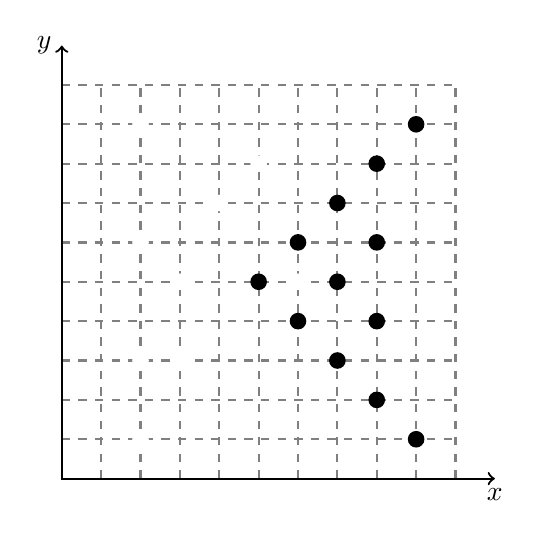
\begin{tikzpicture}
  \draw [thick, color=gray, step=0.5cm, dashed] (0,0) grid (5,5);
  \draw [<->,thick] (0,5.5) node (yaxis) [left] {$y$} |- (5.5,0) node (xaxis) [below] {$x$};
  \foreach \Point in { (4.5,0.5), (4,1), (3.5,1.5), (3,2), (4,2), (2.5,2.5), (3.5,2.5), (3,3), (4,3), (3.5,3.5), (4,4), (4.5,4.5) } {
	\fill[black] \Point circle (3pt);
  }
  \foreach \Point in {(1,0.5), (1,1.5), (1.5,1.5), (1.5,2.5), (1,3), (2,3.5), (2.5,4), (1,4.5), (3, 2.5)} {
    \fill[white] \Point circle (3pt);
  }
\end{tikzpicture}
\caption{Training Sample}\label{fig1}
\end{figure}

\vfill

\subsection*{Solution}

\begin{table}[H]\centering
\begin{tabular}{r l c c}
Kernel & Function Name & Training Error & Execution Time\\
\hline
Linear & \texttt{vanilladot} & 4.761905 & 0.01\\
Radial Basis & \texttt{rbfdot} & 4.761905 & 0.02\\
Polynomial & \texttt{polydot} & 4.761905 & 0.01\\
ANOVA RBF & \texttt{anovadot} & 4.761905 & 0.02\\
Bessel & \texttt{besseldot} & 4.761905 & 0.00\\
Laplacian & \texttt{laplacedot} & 4.761905 & 0.02\\
Spline & \texttt{splinedot} & 9.52381 & 0.01\\
Hyperbolic Tangent & \texttt{tanhdot} & 19.04762 & 0.00\\
\hline
\end{tabular}
\caption{Performance of Different Kernel Functions on Training Sample given in Fig \ref{fig1}}\label{tab1}
\end{table}

The training dataset shown in Figure \ref{fig1} is constructed in comma-separated value format.
Using R programming-language, the training dataset is imported to workspace and is used to construct classifiers using kernels available in the \texttt{kernlab} package.
Table \ref{tab1} provides the list of kernels used for SVM-based classification as well as their training error and execution time for their construction over given training dataset.

Fig \ref{fig2}, generated by R, presents the training error resulting construction of  classifiers using different kernel functions.
As can be seen, \texttt{splinedot} and \texttt{tanhdot} kernels have failed to classify the training dataset accurately.
The similar training error achieved by other kernel functions can be justified by noting the limited amount of samples in the training dataset as well as the way they are formed  which makes it fairly easy to classify.

\begin{figure}\centering
\includegraphics[width=0.8\textwidth]{\imgDirectory/umb-cs671-2015s-f01-02.png}
\caption{Training Error for Different Kernels}\label{fig2}
\end{figure}

Also, plot of execution time of different kernel functions in constructing classifier for the training dataset is given in Figure \ref{fig3}.

\begin{figure}\centering
\includegraphics[width=0.8\textwidth]{\imgDirectory/umb-cs671-2015s-f01-03.png}
\caption{Execution Time for Different Kernel Functions}\label{fig3}
\end{figure}

Figure \ref{fig4} depicts the execution time based on training error for different kernel functions.

\begin{figure}\centering
\includegraphics[width=0.8\textwidth]{\imgDirectory/umb-cs671-2015s-f01-04.png}
\caption{Execution-Time based on Error-Rate for Different Kernels}\label{fig4}
\end{figure}

It can be inferred that using kernel functions that promise better performance in terms of training error might necessitate higher computational costs which lead to longer execution times.
However, this particular example does not prove this point as can be seen in Fig \ref{fig4}.
In fact, rerunning the same script would give different results each time.
This is due to the limited amount of the training dataset that will make the errors in measurement of the execution time quite considerable.
To prove our claim, the same code in R programming language has been applied to the larger database given for letter recognitions, results of which are included in the files attached to this document.

The code in R data-analysis software to construct and compare classifiers over the training dataset given in \ref{fig1} has been given as appendix to this report.

%%%%%%%%%%%%%%%%%%%%%%%%%%%%%%%%%%%%%%%%%%%%%%%%%%%%%%%%%%%%%%%%%%%%%%
% CS630: Database Management Systems
% Copyright 2014 Pejman Ghorbanzade <mail@ghorbanzade.com>
% Creative Commons Attribution-ShareAlike 4.0 International License
% More info: https://bitbucket.org/ghorbanzade/umb-cs630-2014f
%%%%%%%%%%%%%%%%%%%%%%%%%%%%%%%%%%%%%%%%%%%%%%%%%%%%%%%%%%%%%%%%%%%%%%

\section*{Question 3}

Using the schema above, and assuming that grade is of type integer, provide the SQL statement to create a view \texttt{TopStudents} that lists the student ID, name and average grade (GPA) for students that have GPA above 3.0.

\textbf{Solution:}

\lstset{language=SQL}
\lstset{numbers=none}
\begin{lstlisting}
CREATE VIEW TopStudents(sid, sname, GPA) AS
SELECT TMP.sid, TMP.sname, TMP.gpa
FROM (
	SELECT S.sid, S.sname, SUM(C.credits*G.grade)/COUNT(*) AS gpa
	FROM Students S, Courses C, Grades G
	WHERE G.sid = S.sid AND G.cid = C.cid
	GROUP BY S.sid, S.name
	) TMP
WHERE TMP.gpa > 3.0;
\end{lstlisting}

%%%%%%%%%%%%%%%%%%%%%%%%%%%%%%%%%%%%%%%%%%%%%%%%%%%%%%%%%%%%%%%%%%%%%%
% CS671: Machine Learning
% Copyright 2015 Pejman Ghorbanzade <pejman@ghorbanzade.com>
% Creative Commons Attribution-ShareAlike 4.0 International License
% More info: https://github.com/ghorbanzade/beacon
%%%%%%%%%%%%%%%%%%%%%%%%%%%%%%%%%%%%%%%%%%%%%%%%%%%%%%%%%%%%%%%%%%%%%%

\newpage

\section*{Appendices}

\subsection*{Source Code for Question 2}

\lstset{language=r,tabsize=4}
\lstinputlisting[firstline=1]{
	\srcDirectory/r/f01.r
}


\end{document}
